% You should give sufficient motivation to the problem you are dealing with,
% present the background, the options you had in attacking the problem, and the
% reasons you are following some specific policies in your research. This is a
% non-exhaustive list. Depending on the project, you can think of various
% additional aspects to present (e.g., what results would be considered good and
% what bad, etc.).

\documentclass{beamer}

\usepackage{beamerthemesplit}
\usepackage{fancyvrb}

\defbeamertemplate{footline}{author and page number}{%
  \usebeamercolor[fg]{page number in head/foot}%
  \usebeamerfont{page number in head/foot}%
  \hspace{1em}\insertshortauthor\hspace{.5em}--\hspace{.5em}\inserttitle\hfill%
  \insertpagenumber\,/\,\insertpresentationendpage\kern1em\vskip2pt%
}

\setbeamertemplate{footline}[author and page number]{}
\setbeamertemplate{navigation symbols}{}

\title{A Cloud-based Application Storage Service for Ibis}
\author{Bas Boterman}
\date{\today}

\begin{document}

\frame
{
	\titlepage
	\begin{figure}[h]
	\begin{center}
	
\includegraphics[width=2cm]{msc_logo.png} 
	\end{center}
	\end{figure}
}

\section[Outline]{}
\frame
{
	\frametitle{Outline}
	\tableofcontents
}

\section{Introduction}
%\subsection{Background}
\frame
{
	\frametitle{Background}
	\begin{itemize}
    	\item <1->April 7, 2008, the Google App Engine, a platform for developing
    		and hosting web applications, was introduced
    	\item <2->To what extent can we use the Google App Engine for scientific
      		purposes?
      	\item <3->Robust distributed datastore with transactions and queries
    	\item <4->This project is about designing an application storage server
    		for Ibis
    \end{itemize}
}


%\subsection{Thesis}
\frame[t]
{
	\frametitle{Thesis Title}
	A Cloud-based Application Storage Service for Ibis 
}

\frame[t]
{
	\frametitle{Thesis Title}
	A \textbf{Cloud-based} Application Storage Service for Ibis
	\newline
	\uncover<2->{
		\begin{quote}
			``A style of computing in which dynamically scalable resources are provided
			as a service over the Internet.''
		\end{quote}
	
		E.g. the Google App Engine.
	}
}

\frame[t]
{
	\frametitle{Thesis Title}
	A Cloud-based \textbf{Application Storage Service} for Ibis
	\newline
	\uncover<2->{
		\begin{quote}
			``A service used by applications to store and retrieve application data.''
		\end{quote}
		
		Example:
		\begin{figure}[t]
		\begin{center}
		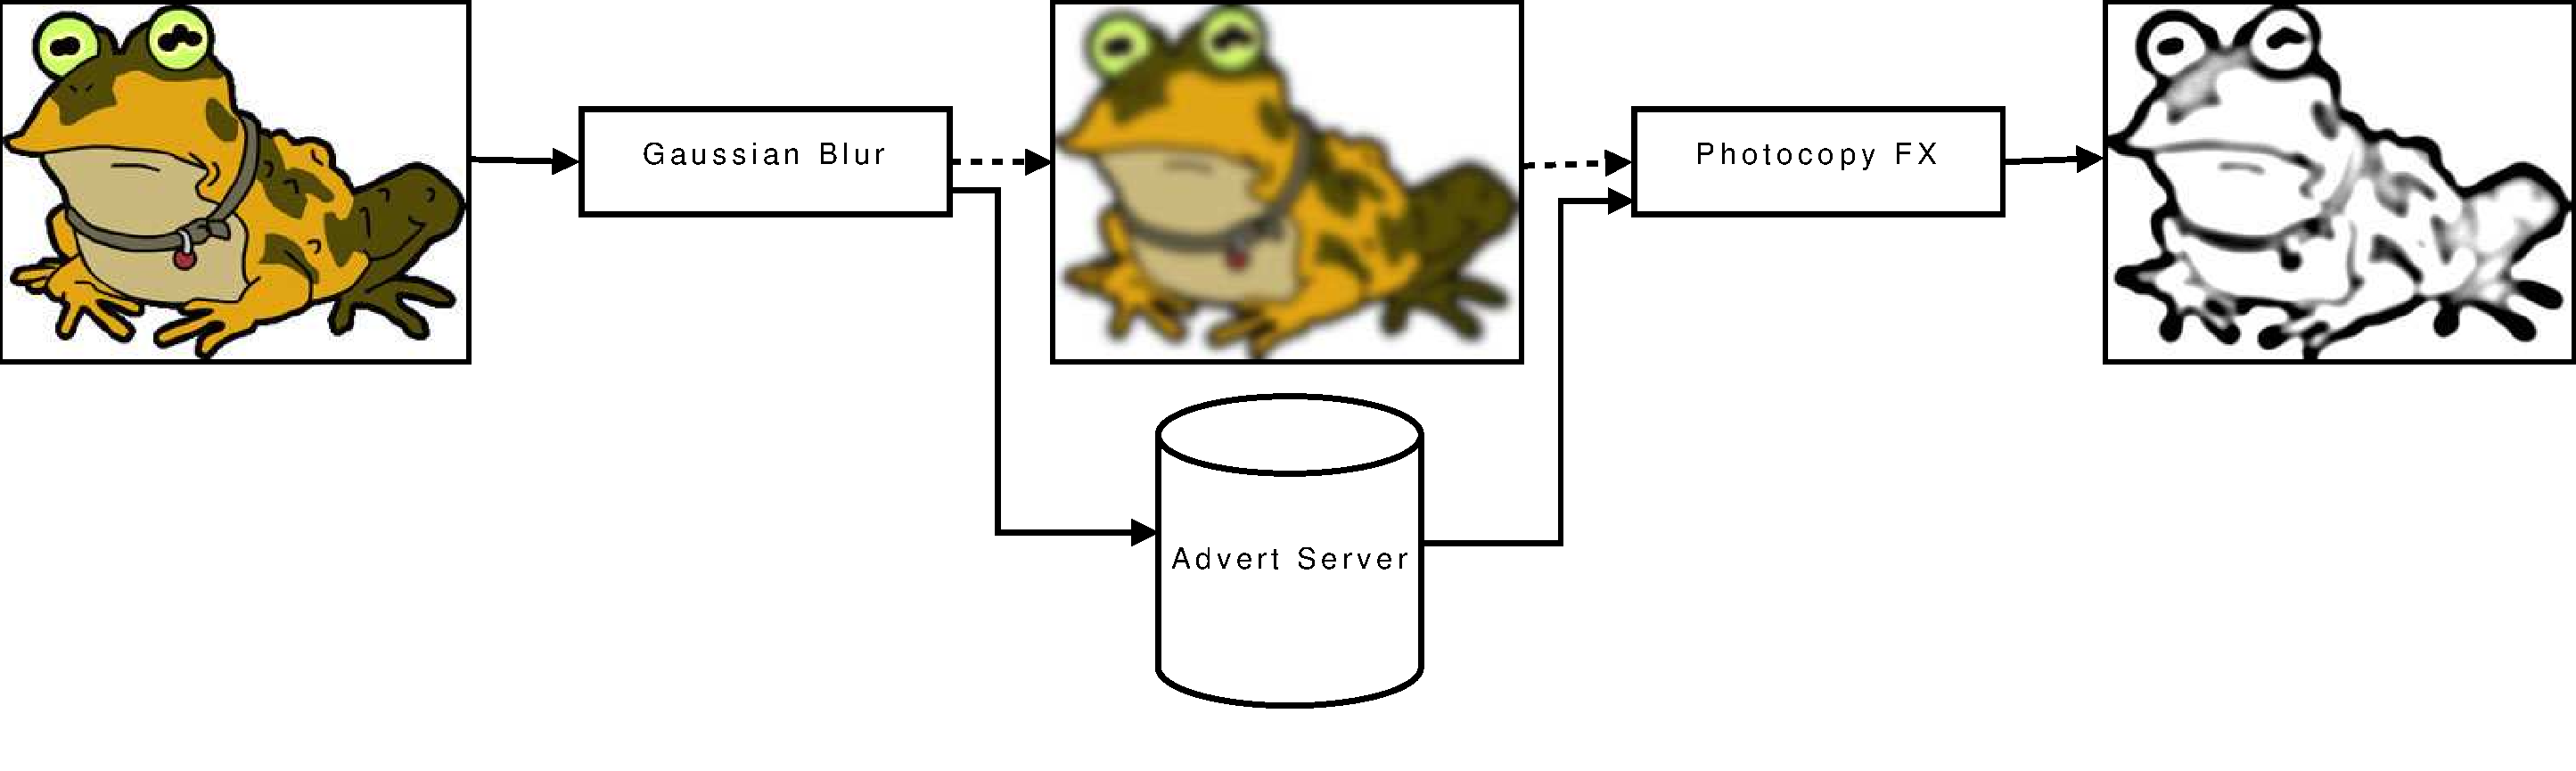
\includegraphics[width=10cm]{image_workflow.pdf} 
		\end{center}
		\end{figure}
	}
}

\frame[t]
{
	\frametitle{Thesis Title}
	A Cloud-based Application Storage Service for \textbf{Ibis}
	\newline
	\uncover<2->{
		\begin{quote}
			``The main goal of the Ibis project is to create an efficient Java-based
			platform for grid computing.''
		\end{quote}
	}
	\begin{itemize}
		\item<2-> JavaGAT (Grid Application Toolkit)
		\item<2-> IPL (Ibis Portability Layer)
	\end{itemize}
}

%\subsection{Google App Engine}
\frame
{
	\frametitle{Google App Engine}
	\begin{quote}
		``A platform for building and hosting web applications on
		the Google infrastructure.''
	\end{quote}
	
	\begin{itemize}
		\item Python programming language
		\item Web application framework
		\item Authentication through Google Accounts
		\item Free of charge
		\begin{itemize}
			\item 10\,GB traffic per day
			\item 1\,GB of data storage
		\end{itemize}
	\end{itemize}
}

%\subsection{Properties}
\frame
{
	\frametitle{(Dis)Advantages of the Google App Engine}
	\uncover<1->{Advantages:}
	\begin{itemize}
		\item <1->Powerful (distributed) database with query engine and
			transactions
		\item <1->Replicating servers to improve scalability 
		\item <1->Authentication through Google Accounts
		\item <1->Built-in frameworks (Django, WebOb, PyYAML)
	\end{itemize}

	\uncover<2->{Disadvantages:}
	\begin{itemize}
		\item <2->Python 2.5 (limited functionality, compared to 3.0)
		\item <2->HTTP(S) only
		\item <2->Sandbox (no \texttt{fork()}, no threads, no file system)
	\end{itemize}
}

\section{Project Details}
%\subsection{Design}
\frame
{
	\frametitle{Project Overview}
	\begin{figure}
	\begin{center}
	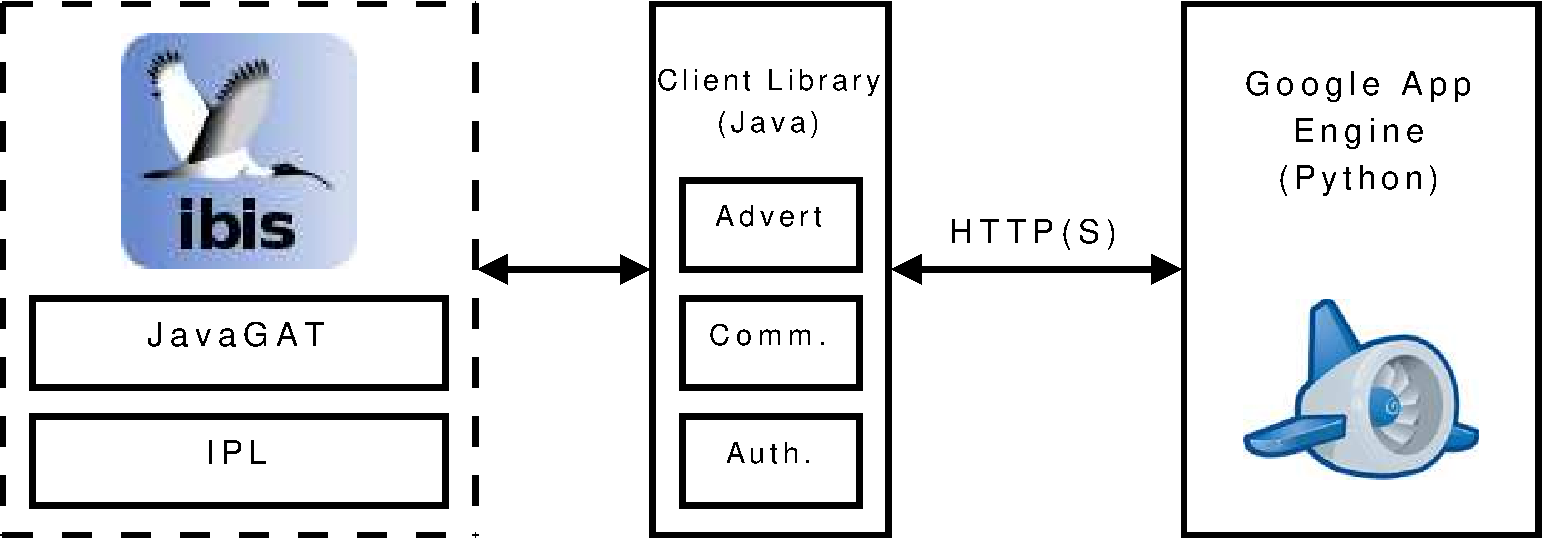
\includegraphics[width=10cm]{proj_design.pdf} 
	\end{center}
	\end{figure}
}

\frame
{
	\frametitle{Server Design}
	Public functions:
	\begin{itemize}
		\item \texttt{add(data, metadata, path)}
		\item \texttt{del(path)}
		\item \texttt{get(path)}
		\item \texttt{getmd(path)}
		\item \texttt{find(metadata)}
	\end{itemize}
	\begin{itemize}
		\item \texttt{data}: Text
		\item \texttt{metadata}: Key-value pairs of Strings
		\item \texttt{path}: String
	\end{itemize}
}

\frame
{
	\frametitle{Client Library}
	\begin{itemize}
		\item Written in Java
		\item Implements the Google App Engine Advert server's protocol
		\begin{itemize}
			\item Base64 encoding
			\item JSON encoding (XML alternative)
			\item Error handling 
        \end{itemize}
        \item Establishes connections over HTTP(S)
		\item Takes care of authentication
		\begin{itemize}
			\item Authentication through \emph{Google ClientLogin}
			\item Automatically refresh authentication cookie
		\end{itemize} 
	\end{itemize}
}

\section{Benchmarks}
%\subsection{Server Functions}
\frame
{
	\frametitle{Adding Objects of Variable Size}
	\begin{figure}[t]
	\begin{center}
	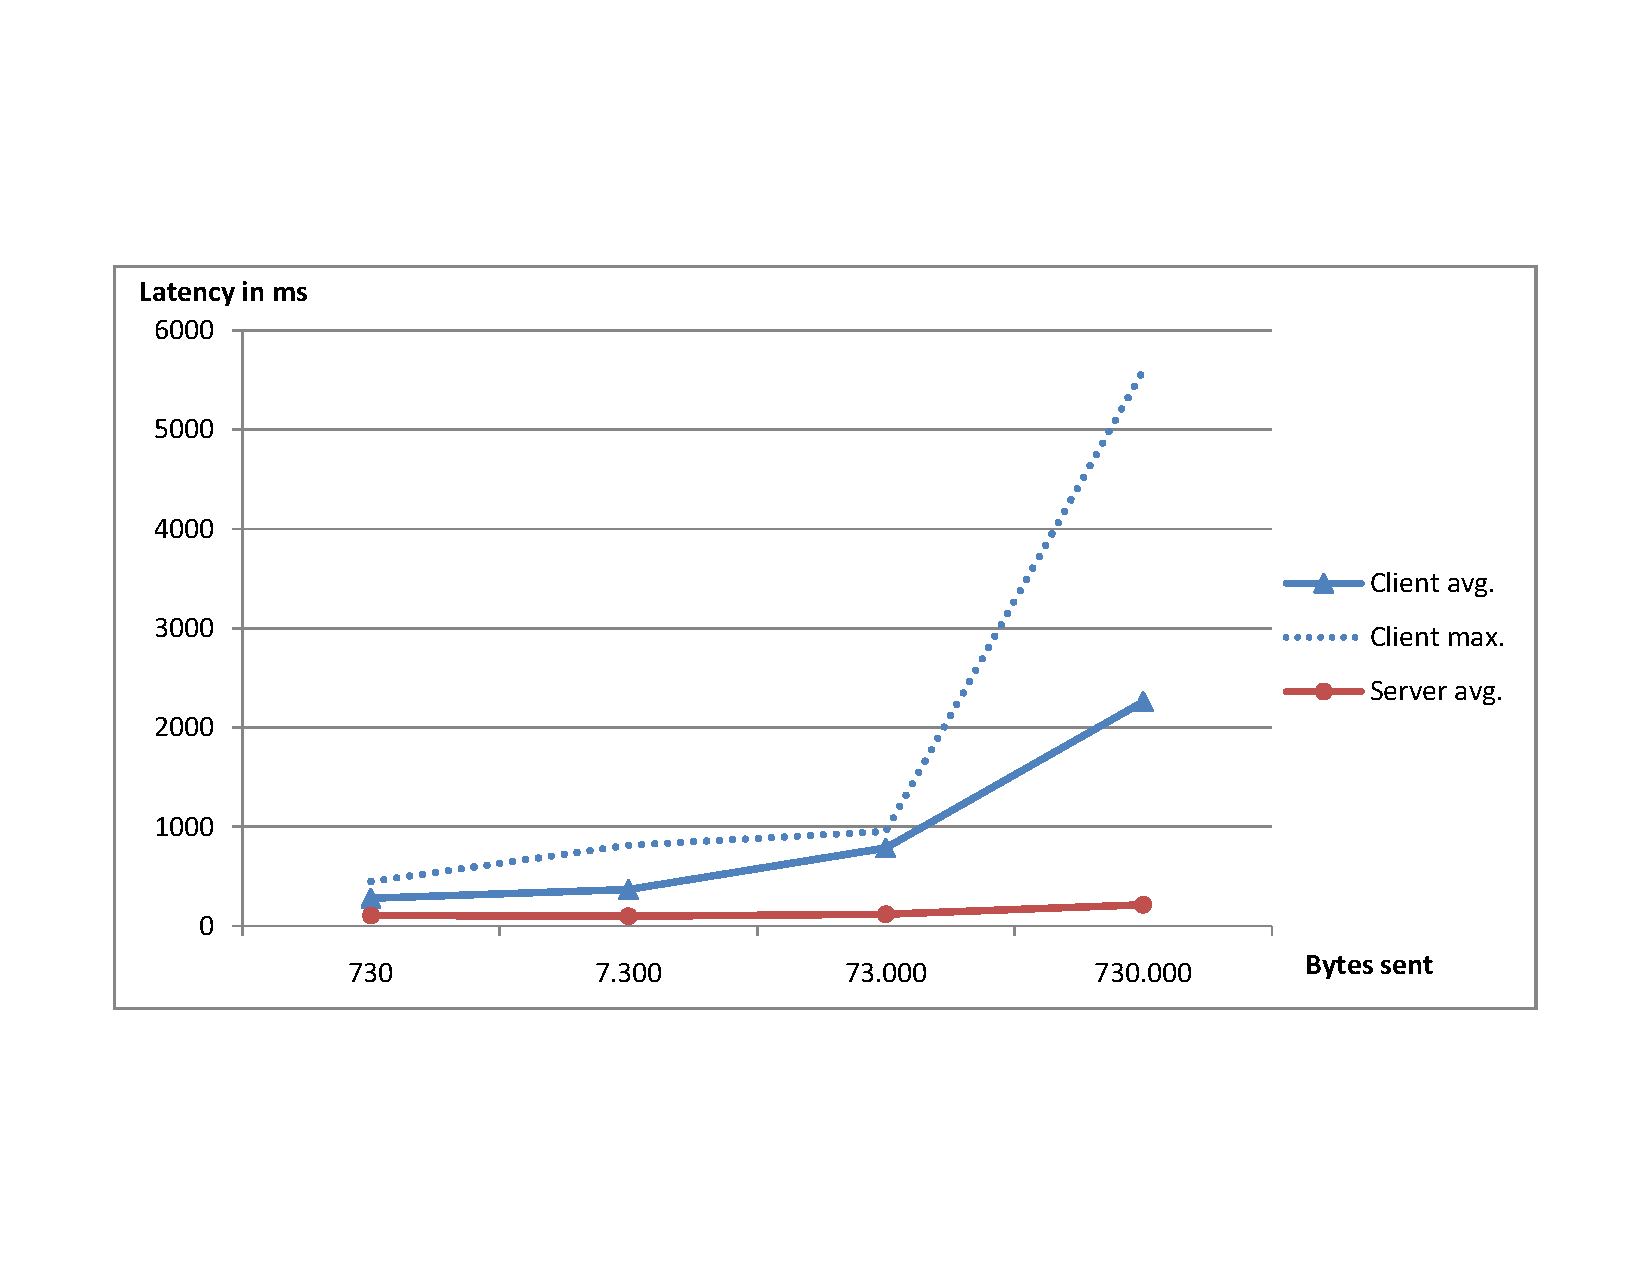
\includegraphics[trim=4cm 4cm 4cm 5cm, width=10cm]{add_obj.pdf} 
	\end{center}
	\end{figure}
}

\frame
{
	\frametitle{Adding Objects with Variable Meta Data}
	\begin{figure}[t]
	\begin{center}
	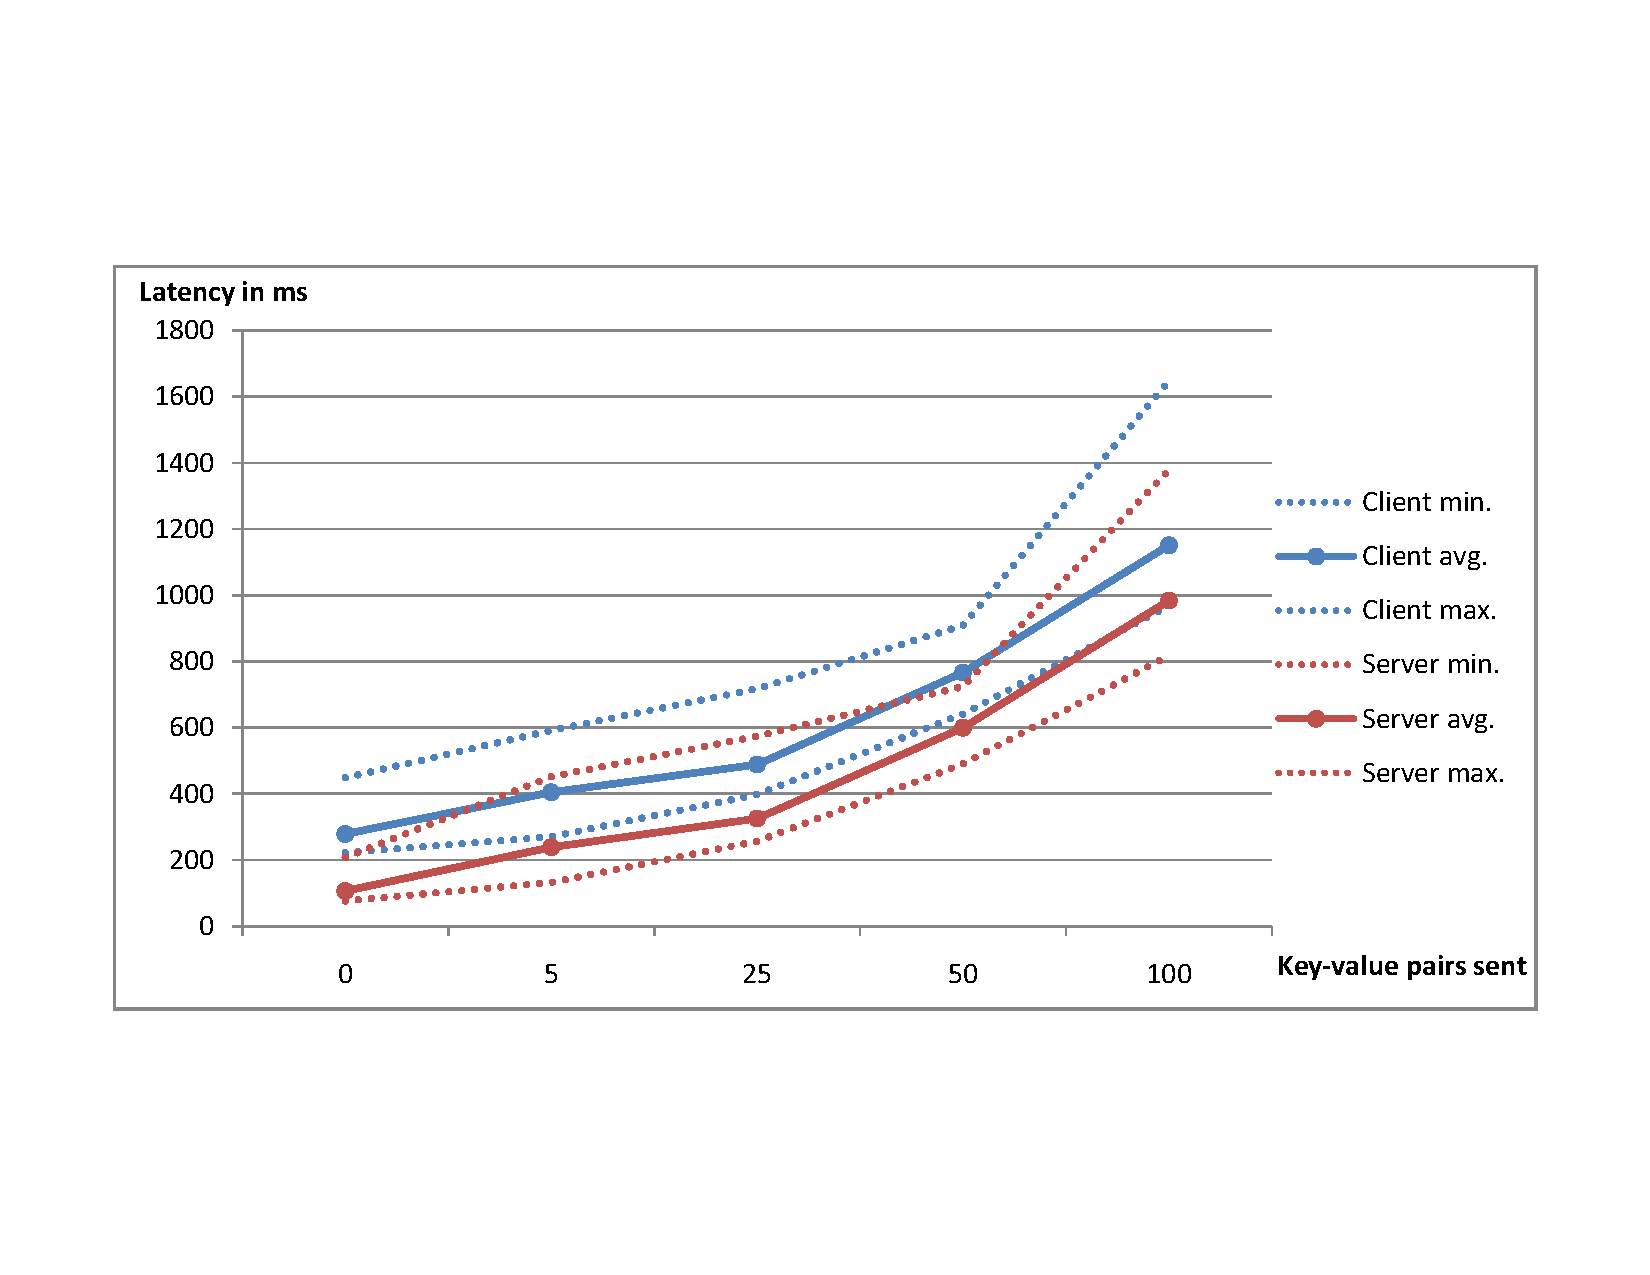
\includegraphics[trim=4cm 4cm 4cm 5cm, width=10cm]{add_md.pdf} 
	\end{center}
	\end{figure}
}

\frame
{
	\frametitle{Retrieving Objects with Variable Datastore Size}
	\begin{figure}[t]
	\begin{center}
	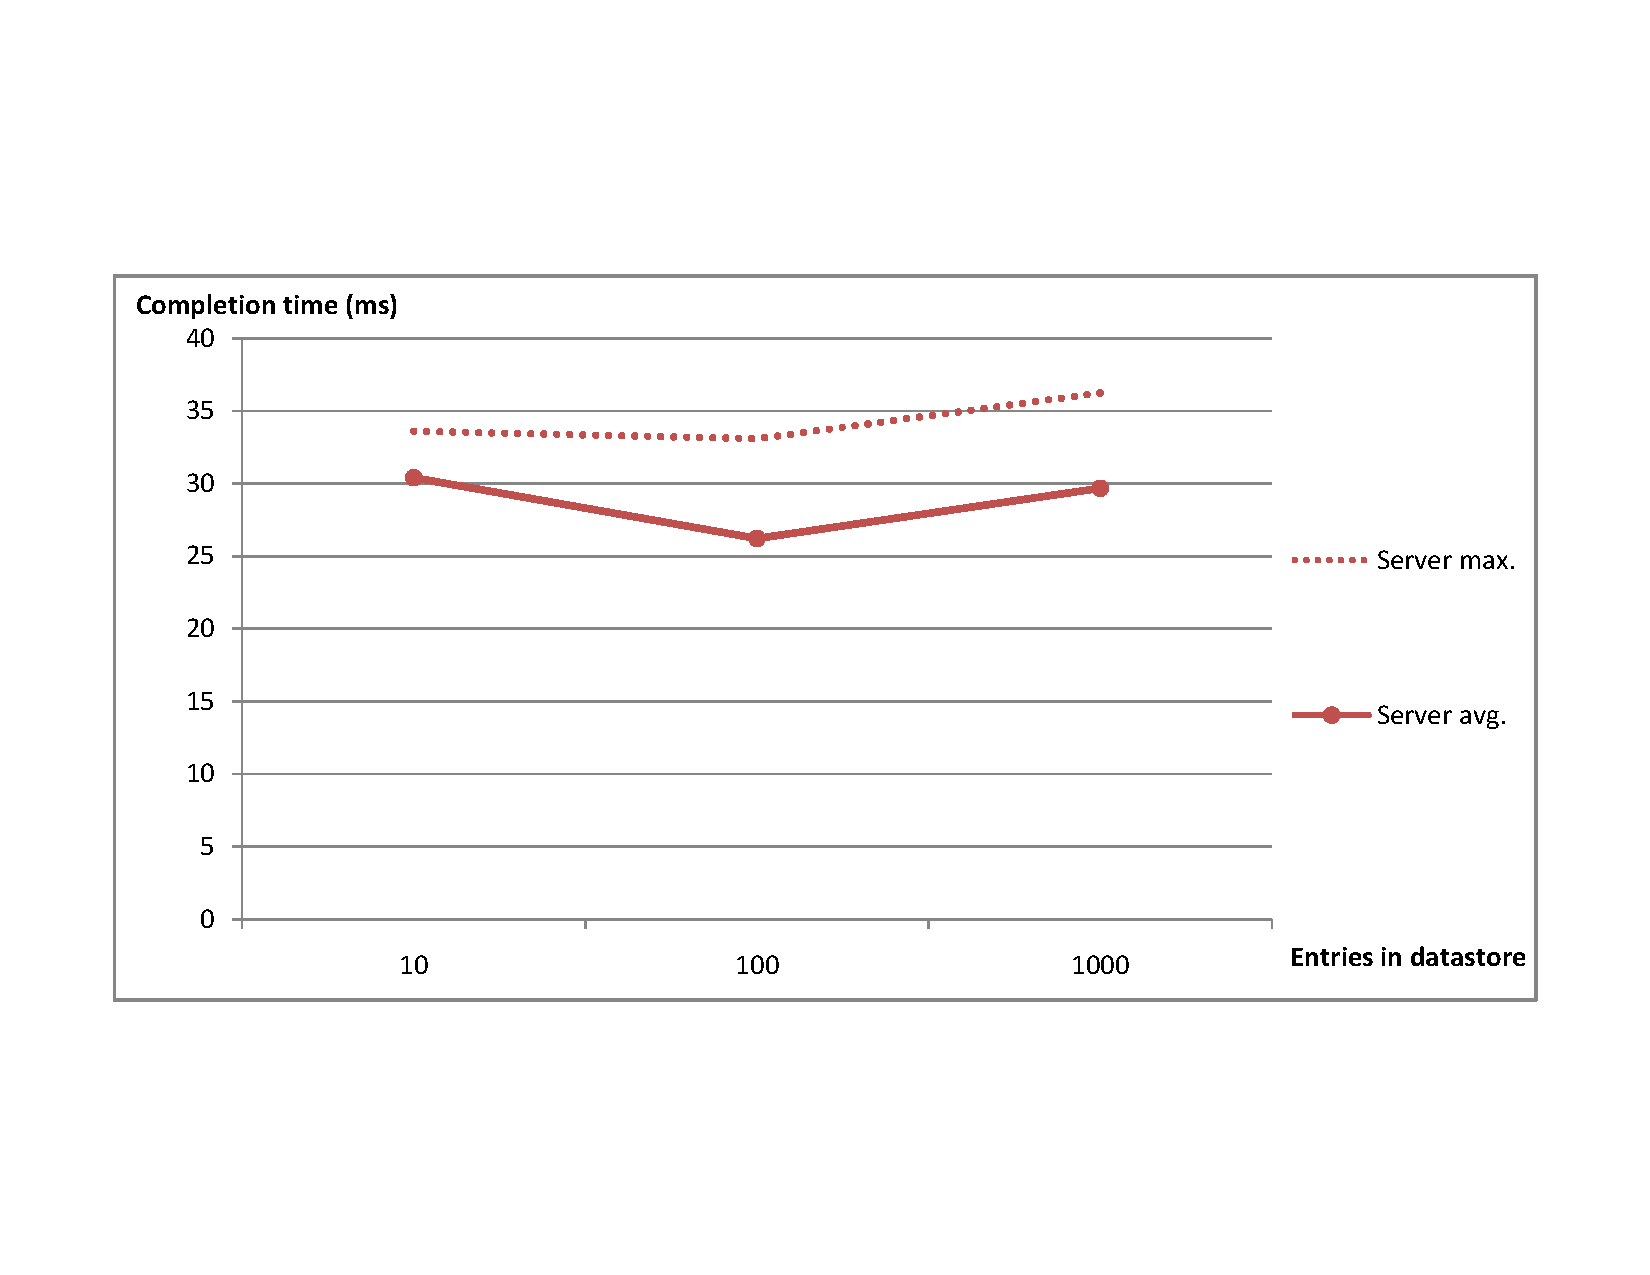
\includegraphics[trim=4cm 4cm 4cm 5cm, width=10cm]{get_amt.pdf} 
	\end{center}
	\end{figure}
}

\frame
{
	\frametitle{Finding Meta Data}
	\begin{figure}[t]
	\begin{center}
	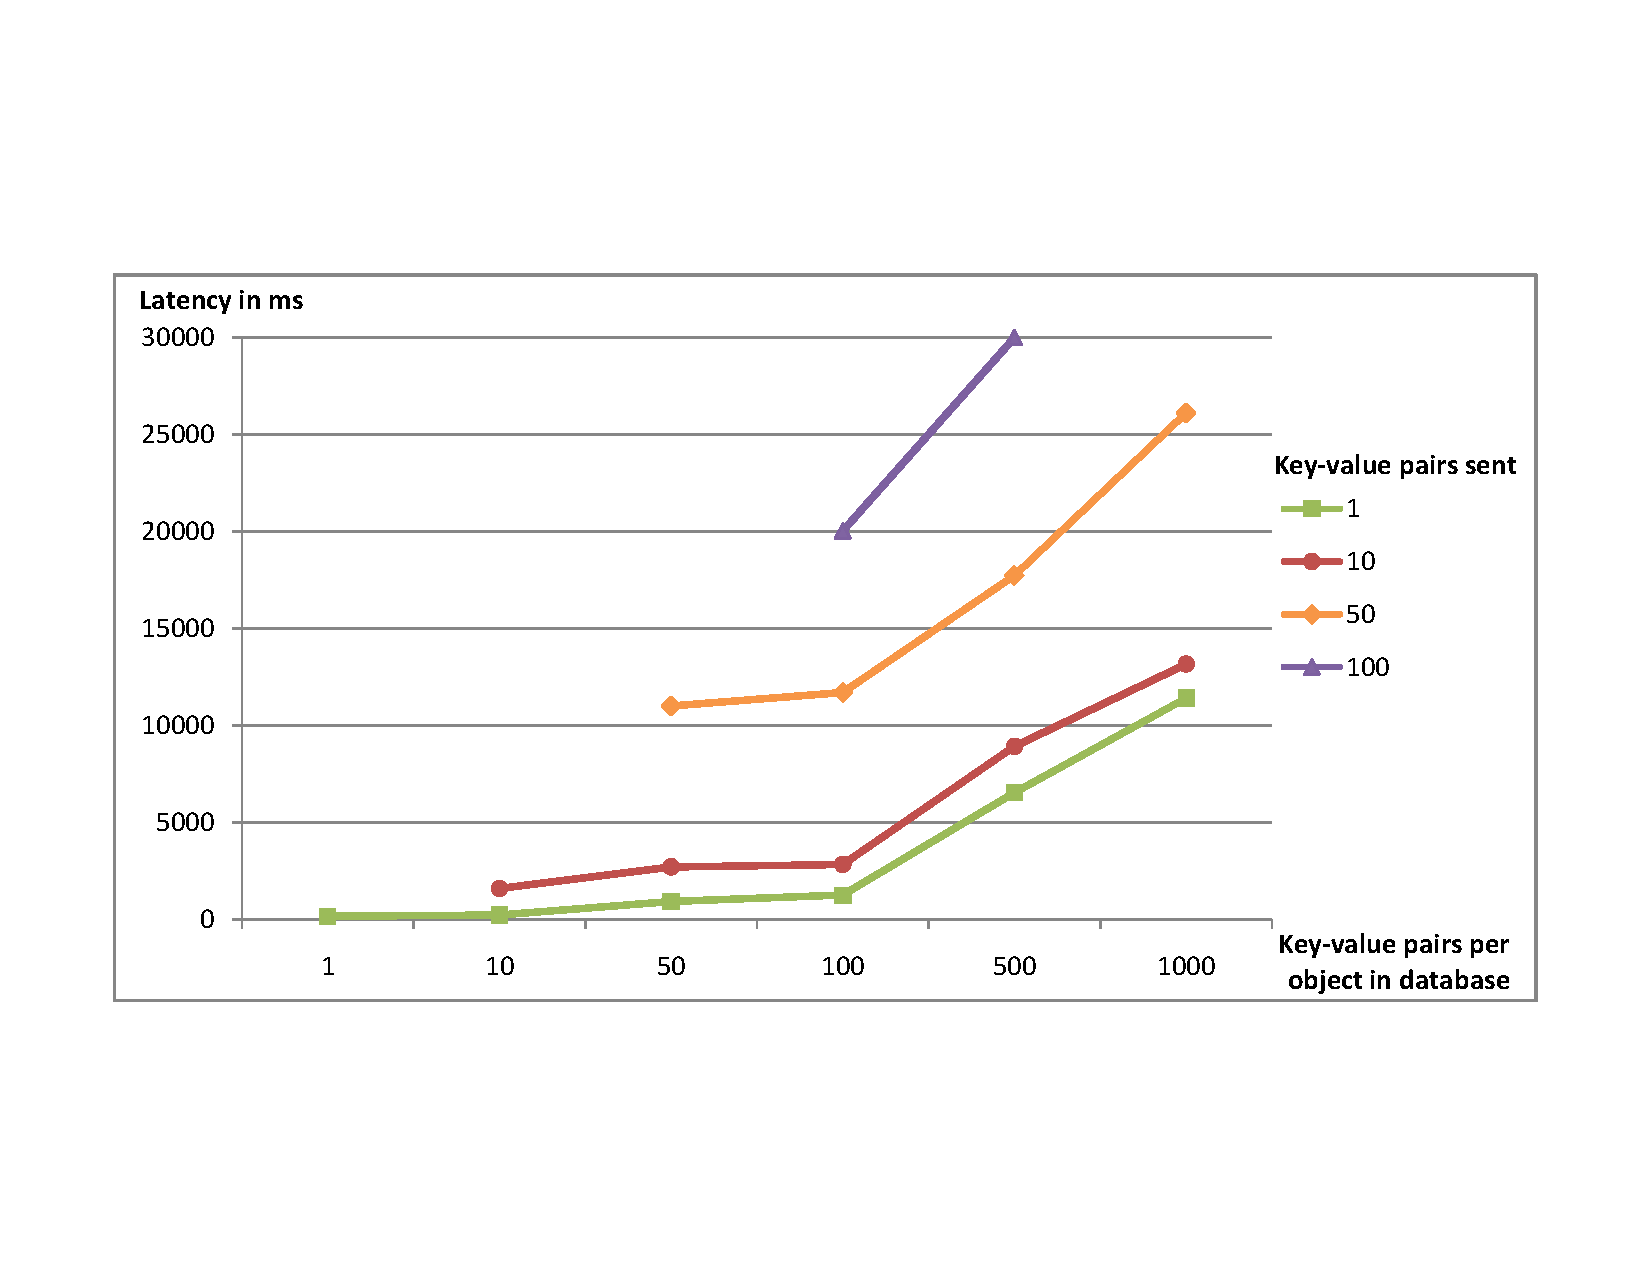
\includegraphics[trim=4cm 4cm 4cm 5cm, width=10cm]{find_amt.pdf} 
	\end{center}
	\end{figure}
}

%\subsection{Clients in Parallel}
\frame
{
	\frametitle{Performing Operations in Parallel}
	\begin{figure}[t]
	\begin{center}
	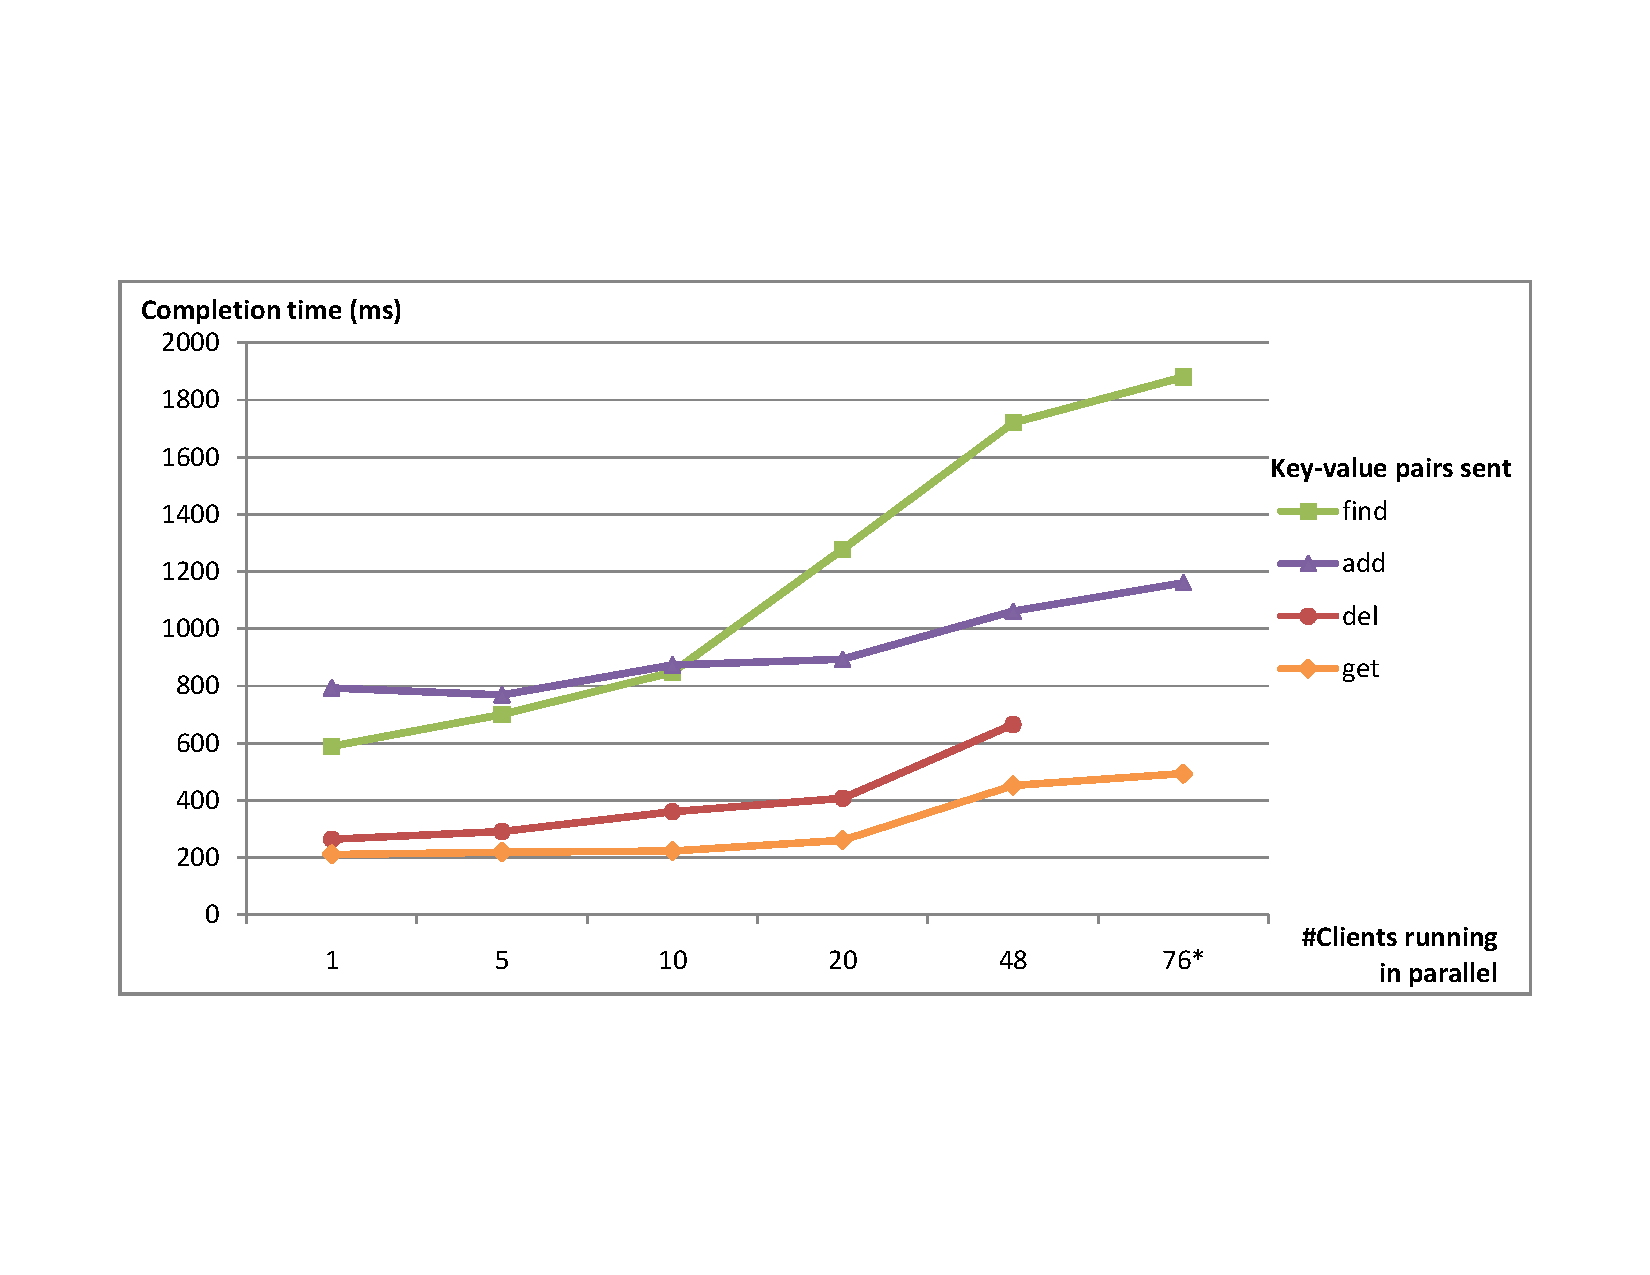
\includegraphics[trim=4cm 4cm 4cm 5cm, width=10cm]{parallel.pdf} 
	\end{center}
	\end{figure}
}

\frame
{
	\frametitle{Benchmark Evaluation}
	\begin{itemize}
    	\item Completion time depends on object size/meta data size, and on number
    		of clients connecting simultaneously
    	\item Completion time is independent on the datastore size
    	\item Google has some restrictions
		\begin{itemize}
    		\item Response time cannot be over 30\,seconds
    		\item Quota temporarily exceeds with requests larger than 5\,MB
    		\item No more than 500 data items can be manipulated in one call
    		\item No more than 100 clients can use ClientLogin simultaneously
    	\end{itemize}
    \end{itemize}
}

\section{Applications}
\frame
{
	\frametitle{Outline}
	\tableofcontents[currentsection]
}

%\subsection{JavaGAT}
\frame
{
	\frametitle{JavaGAT}
	\begin{quote}
		JavaGAT offers a set of coordinated, generic and flexible APIs for accessing
		grid services from application codes, portals, data managements systems, etc.
	\end{quote}
	
	\begin{itemize}
		\item File operations
		\item Job submission
		\item Monitoring
		\item Access to information services (AdvertService)
	\end{itemize}
}

\frame[t]
{
	\frametitle{JavaGAT structure}
	\begin{figure}[t]
	\begin{center}
	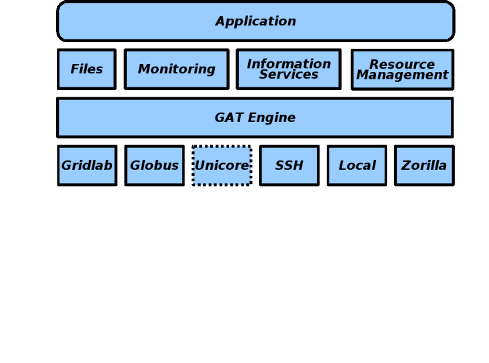
\includegraphics[width=7cm]{gat-design.png} 
	\end{center}
	\end{figure}
}

\frame[t]
{
	\frametitle{JavaGAT structure with App Engine AdvertService Adaptor}
	\begin{figure}[t]
	\begin{center}
	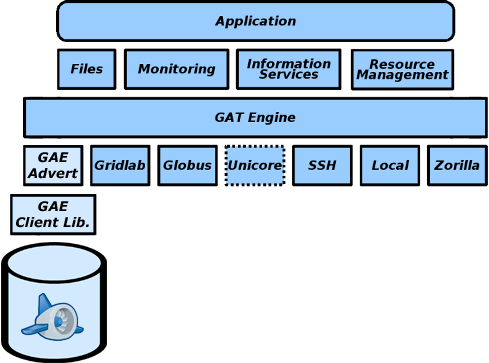
\includegraphics[width=7cm]{gat-mydesign.png} 
	\end{center}
	\end{figure}
}

\frame
{
	\frametitle{App Engine AdvertService Adaptor}
	\begin{itemize}
		\item So far, only a local AdvertService existed
		\item Scalable design (local AdvertService does not scale)
		\item Completely transparent to user
		\item Path handling is done locally
    \end{itemize}
}

%\subsection{IPL}
\frame
{
	\frametitle{IPL (Ibis Portability Layer)}
	\begin{quote}
		``The IPL is a communication library which is specifically designed for usage
		in a grid environment.''
	\end{quote}
	\begin{itemize}
    	\item Communication library for distributed applications
    	\item All applications discover each other through an IPL registry server
    	\item IPL registry server address needs to be passed to each Ibis
    		application
    \end{itemize}
}

\frame[t,containsverbatim]
{
	\frametitle{IPL Example}
	\begin{Verbatim}[fontsize=\small,gobble=2]
		$ $IPL_HOME/bin/ipl-server --events

		Ibis server running on 130.37.20.18-8888~bbn230
		List of Services:
		    Bootstrap service on virtual port 303
		    Central Registry service on virtual port 302
		    Management service
		Known hubs now: 130.37.20.18-8888~bbn230
		

		$ $IPL_HOME/bin/ipl-run \
		-Dibis.server.address=130.37.20.18-8888~bbn230 \
		-Dibis.pool.name=test \
		ibis.ipl.examples.Hello
    \end{Verbatim}
}

\frame[t,containsverbatim]
{
	\frametitle{IPL Example Using Advert Server}
	\begin{Verbatim}[fontsize=\small,gobble=2]
		$ $IPL_HOME/bin/ipl-server --events \
		--advert google://jondoe.appspot.com/identifier \
		--user jondoe@gmail.com --pass north23AZ \
		--metadata author=jondoe,created=24jun,pool=test,color=purple

		Ibis server running on 130.37.20.18-8888~bbn230
		List of Services:
		    Bootstrap service on virtual port 303
		    Central Registry service on virtual port 302
		    Management service
		Known hubs now: 130.37.20.18-8888~bbn230
	\end{Verbatim}
}

\frame[t,containsverbatim]
{
	\frametitle{IPL Example Using Advert Server}
	\begin{Verbatim}[fontsize=\small,gobble=2]
		$ $IPL_HOME/bin/ipl-run \
		-Dibis.advert.address=google://jondoe.appspot.com \
		-Dibis.advert.username=jondoe \
		-Dibis.advert.password=north23AZ \
		-Dibis.advert.metadata=created=24jun,color=purple \
		-Dibis.pool.name=test \
		ibis.ipl.examples.Hello
    \end{Verbatim}
}

\frame
{
	\frametitle{IPL Server Bootstrap Mechanism}
	\begin{itemize}
    	\item No mechanism for bootstrapping IPL servers existed
    	\item Large range of IPL servers can be started, whilst only remembering
    		one (advert) address
		\item Different groups of Ibises can be started without (manually) having to
			configure each Ibis %Advert address can be hard-coded in Ibis application 
    \end{itemize}
}

\section{Conclusion}
%\subsection{Verdict}
\frame{
	\frametitle{Conclusion}
	Contributions:
	\begin{itemize}
      \item <1->A Google App Engine Advert server, written in Python
      \item <1->An Advert client library, written in Java
      \item <1->An App Engine AdvertService adaptor for JavaGAT
      \item <1->An IPL Server bootstrap mechanism
    \end{itemize}
	
	\uncover<2->{Properties:}
	\begin{itemize}
      \item <2->Scalable application and datastore
      \item <2->High bandwidth (until quota reached)
      \item <2->No guarantees
    \end{itemize}
    
    \uncover<3->{Future work:}
    \begin{itemize}
      \item <3->An App Engine Advert server, written in Java
    \end{itemize}
}

%\subsection{Questions}
% \frame{
% 	\frametitle{Questions}
% 	\begin{center}
% 		\huge{Any questions?}
% 	\end{center}
% }
\end{document}